\documentclass[conference]{IEEEtran}

\usepackage{graphicx}
\usepackage{booktabs}
\usepackage{url}
\usepackage{array}
\usepackage{float}
\usepackage{amsmath}

\setlength{\emergencystretch}{2em}

\title{SchEDU: Adaptive Academic Pacing Using Deterministic Constraint-Based Greedy Scheduling and Heuristic Rebalancing}

\author{
\IEEEauthorblockN{Aundreka Clarinze Perez, Marjinel Abante, Leo Franklin Borromeo}
\IEEEauthorblockA{
College of Information Technology and Computer Science\\
Lyceum of the Philippines University -- Cavite\\
Cavite, Philippines\\
\{perez.aundreka, abante.marjinel, borromeo.leofranklin\}@lpu.edu.ph
}
}

\begin{document}

\maketitle

\begin{abstract}
Teachers often manage lesson content, class schedules, assessments, school events,
and instructional documents across disconnected tools such as paper planners,
spreadsheets, messaging threads, and cloud file folders. This fragmentation makes
it difficult to maintain a coherent academic plan, especially when classes are
suspended, assessments must be redistributed, or curriculum materials need to be
converted into reusable lesson content. This paper presents SchEDU, an implemented
mobile academic planning system that consolidates these tasks into a single
teacher-facing workflow. SchEDU combines a React Native mobile client, a
Supabase-backed cloud data layer, and a deterministic constraint-based greedy
scheduling pipeline for generating and maintaining lesson-plan calendars. The
system stores structured academic content, generates schedule slots from teacher
meeting patterns, places lesson and assessment blocks according to term rules and
dependency conditions, and rebalances schedules when blackout dates or teaching
disruptions occur. Supporting utilities include curriculum text extraction from
PDF or image uploads and AI-assisted generation of classroom activity documents.
Validation is based on repository-backed implementation inspection, schema and
Edge Function guards, Expo linting, and executable scheduler invariants covering
initial generation, suspension, restoration, idempotency, and locked-block conflict
handling. The practical contribution of SchEDU is a defense-ready, mobile-first
planning workspace that connects curriculum data, generated schedules, calendar
maintenance, and instructional document support.
\end{abstract}

\section{Introduction}

Academic planning at the teacher level requires more than simply recording dates on
a calendar. Teachers must organize subjects, chapters, and lessons; align them with
term dates and recurring class meetings; place written work and performance tasks at
appropriate points in the term; and respond to suspensions, holidays, and absences
without losing pacing continuity. In many schools, these activities are distributed
across separate notebooks, spreadsheet templates, messaging channels, and document
storage platforms, which increases clerical overhead and makes schedule adjustment
slow and error-prone.

SchEDU was developed to address this fragmentation through a single mobile
application that integrates content management, lesson planning, schedule
generation, disruption handling, and supporting document workflows. Rather than
targeting institution-wide room allocation or full university timetabling, SchEDU
focuses on teacher-facing instructional planning. Its central scheduling problem is
to translate structured lesson content and recurring meeting patterns into a usable
term calendar while respecting exam timing, blackout dates, teacher locks, and
assessment distribution rules.

The current version is not merely a conceptual model. It is an Expo Router and
React Native application with authenticated screens, Supabase-backed persistence,
repository-local scheduling modules, calendar maintenance flows, document
extraction support, and AI-assisted activity generation. This implementation
status matters for evaluation because the system can be demonstrated live: a
teacher can authenticate, manage academic records, generate a plan, inspect the
calendar, trigger a disruption, and observe deterministic schedule maintenance.

The system follows a client-server architecture built on Expo Router, React Native,
and Supabase services. Its scheduling engine is deterministic and
constraint-based: meeting patterns produce candidate instructional slots, lesson
and assessment blocks are generated from stored academic content and term rules,
blocks are greedily placed and ordered on the calendar, and schedule rebalancing
is triggered when class-day availability changes.

The contributions of this paper are the following:
\begin{itemize}
\item a mobile academic planning interface for teacher workflows;
\item a structured academic-content repository spanning schools, sections, subjects,
units, chapters, lessons, and lesson plans;
\item a deterministic constraint-based greedy schedule generation and heuristic
calendar rebalance pipeline built for teacher lesson planning;
\item integrated handling of blackout dates, suspensions, and teacher-locked
schedule edits; and
\item support services for curriculum text extraction and AI-assisted activity
document generation; and
\item a repository-backed validation package covering scheduler invariants,
schema constraints, protected Edge Functions, lint output, and live demonstration
scenarios.
\end{itemize}

\section{Related Work}

\subsection{Teacher Planning and Curriculum Management}

Curriculum implementation requires teachers to adapt prescribed content to local
teaching conditions, available class time, and disruptions in school operations
\cite{pak2020}. This makes planning an ongoing maintenance task rather than a
one-time document preparation activity. Systems that support teacher planning
therefore benefit from representing both instructional content and calendar context
in a structured form.

\subsection{Educational Scheduling and Timetabling}

Educational timetabling research has long examined the assignment of academic
activities to constrained time slots \cite{schaerf1999}. However, much of the
literature focuses on institution-wide scheduling problems such as room assignment,
course timetables, or examination scheduling. SchEDU operates at a narrower but
practically important level: teacher-facing lesson-plan scheduling, where the main
concerns are lesson sequencing, assessment placement, blackout handling, and
day-to-day maintenance of an instructional calendar.

\subsection{Mobile and Cloud Academic Information Systems}

Mobile and cloud-backed information systems are well suited for academic workflows
that require persistent access, multi-device synchronization, and role-based data
management. In the case of SchEDU, the mobile client supports planning in the field
while the cloud backend provides authentication, storage, shared academic records,
and server-side utilities.

\subsection{Document Extraction and AI-Assisted Instructional Support}

Teachers also work with semi-structured materials such as curriculum PDFs, scanned
tables of contents, and assessment templates. Extracting reusable text from these
sources and generating first-draft activity documents can reduce repetitive manual
encoding. In SchEDU, these support functions are treated as auxiliary services that
enhance planning workflows rather than replace teacher judgment.

\section{Methodology and System Design}

\subsection{System Architecture}

SchEDU follows a client-server architecture composed of a mobile frontend, a cloud
backend, and scheduling and utility services.

\begin{figure}[t]
\centering
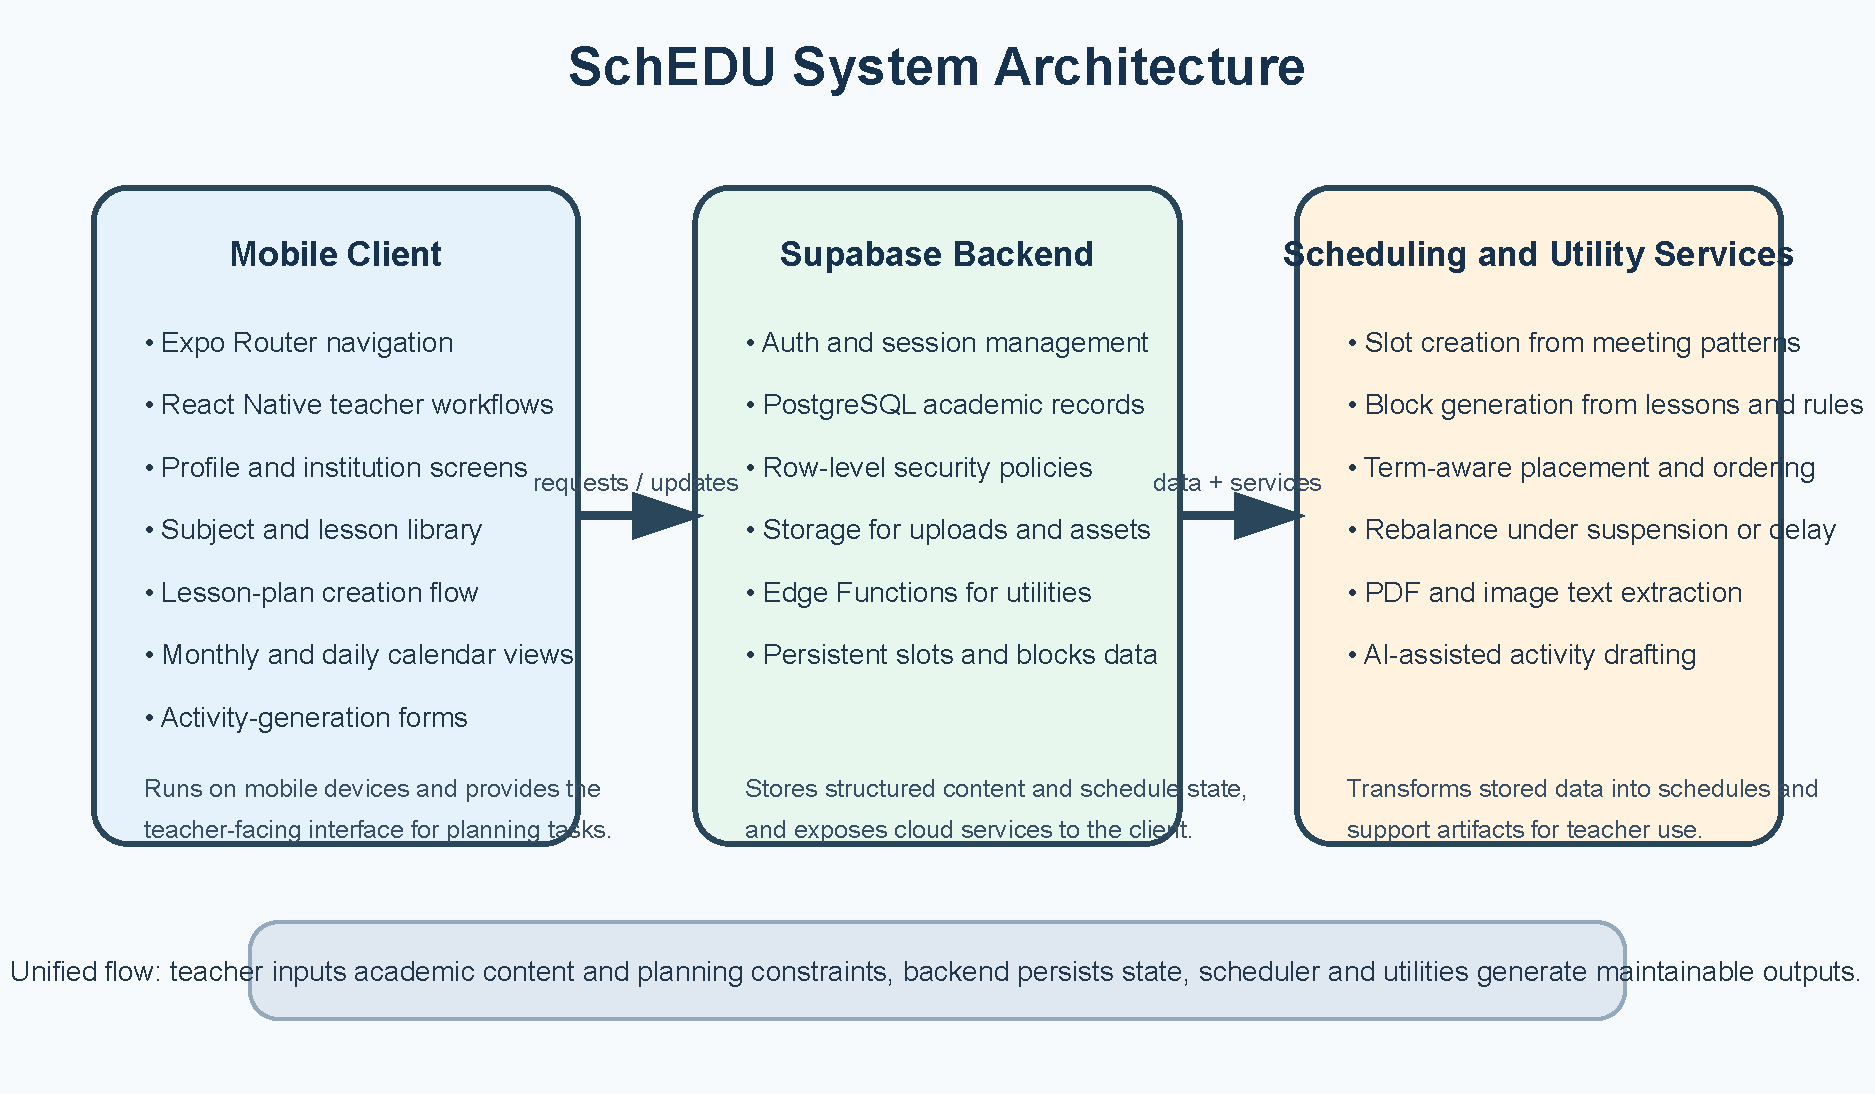
\includegraphics[width=0.48\textwidth]{figures/system-architecture.pdf}
\caption{SchEDU system architecture}
\label{fig:architecture}
\end{figure}

The mobile frontend is implemented with React Native and Expo Router. It provides
teacher-facing workflows for authentication, profile and institution management,
subject and lesson libraries, lesson-plan creation, calendar viewing, and activity
generation. The backend uses Supabase Auth for user access, PostgreSQL for
application data, Storage for uploaded assets, and Edge Functions for selected
server-side utilities.

Figure~\ref{fig:architecture} summarizes the separation of concerns. The client is
responsible for interaction and presentation, the Supabase layer is responsible for
identity, persistence, and controlled access to academic records, and the
scheduling and utility layer is responsible for deriving maintainable outputs from
stored data. This separation is important for a teacher-facing system because it
keeps the mobile application responsive while allowing schedule generation and
document support functions to operate over persistent cloud state.

\subsection{Core Data Model}

The data model represents both academic structure and planning state. User and
institution tables support multi-tenant access across schools and sections. Subject
content is organized hierarchically through subjects, units, chapters, and lessons.
Lesson plans then bind this content to a specific teacher, subject, section, and
date range. Scheduling state is stored through slots, blocks, school calendar
events, and delays.

This structure allows the system to connect content preparation and schedule
execution. Lessons are not stored as isolated notes; they can become scheduled
blocks within a lesson plan and remain linked to term rules and calendar events.

\begin{figure}[t]
\centering
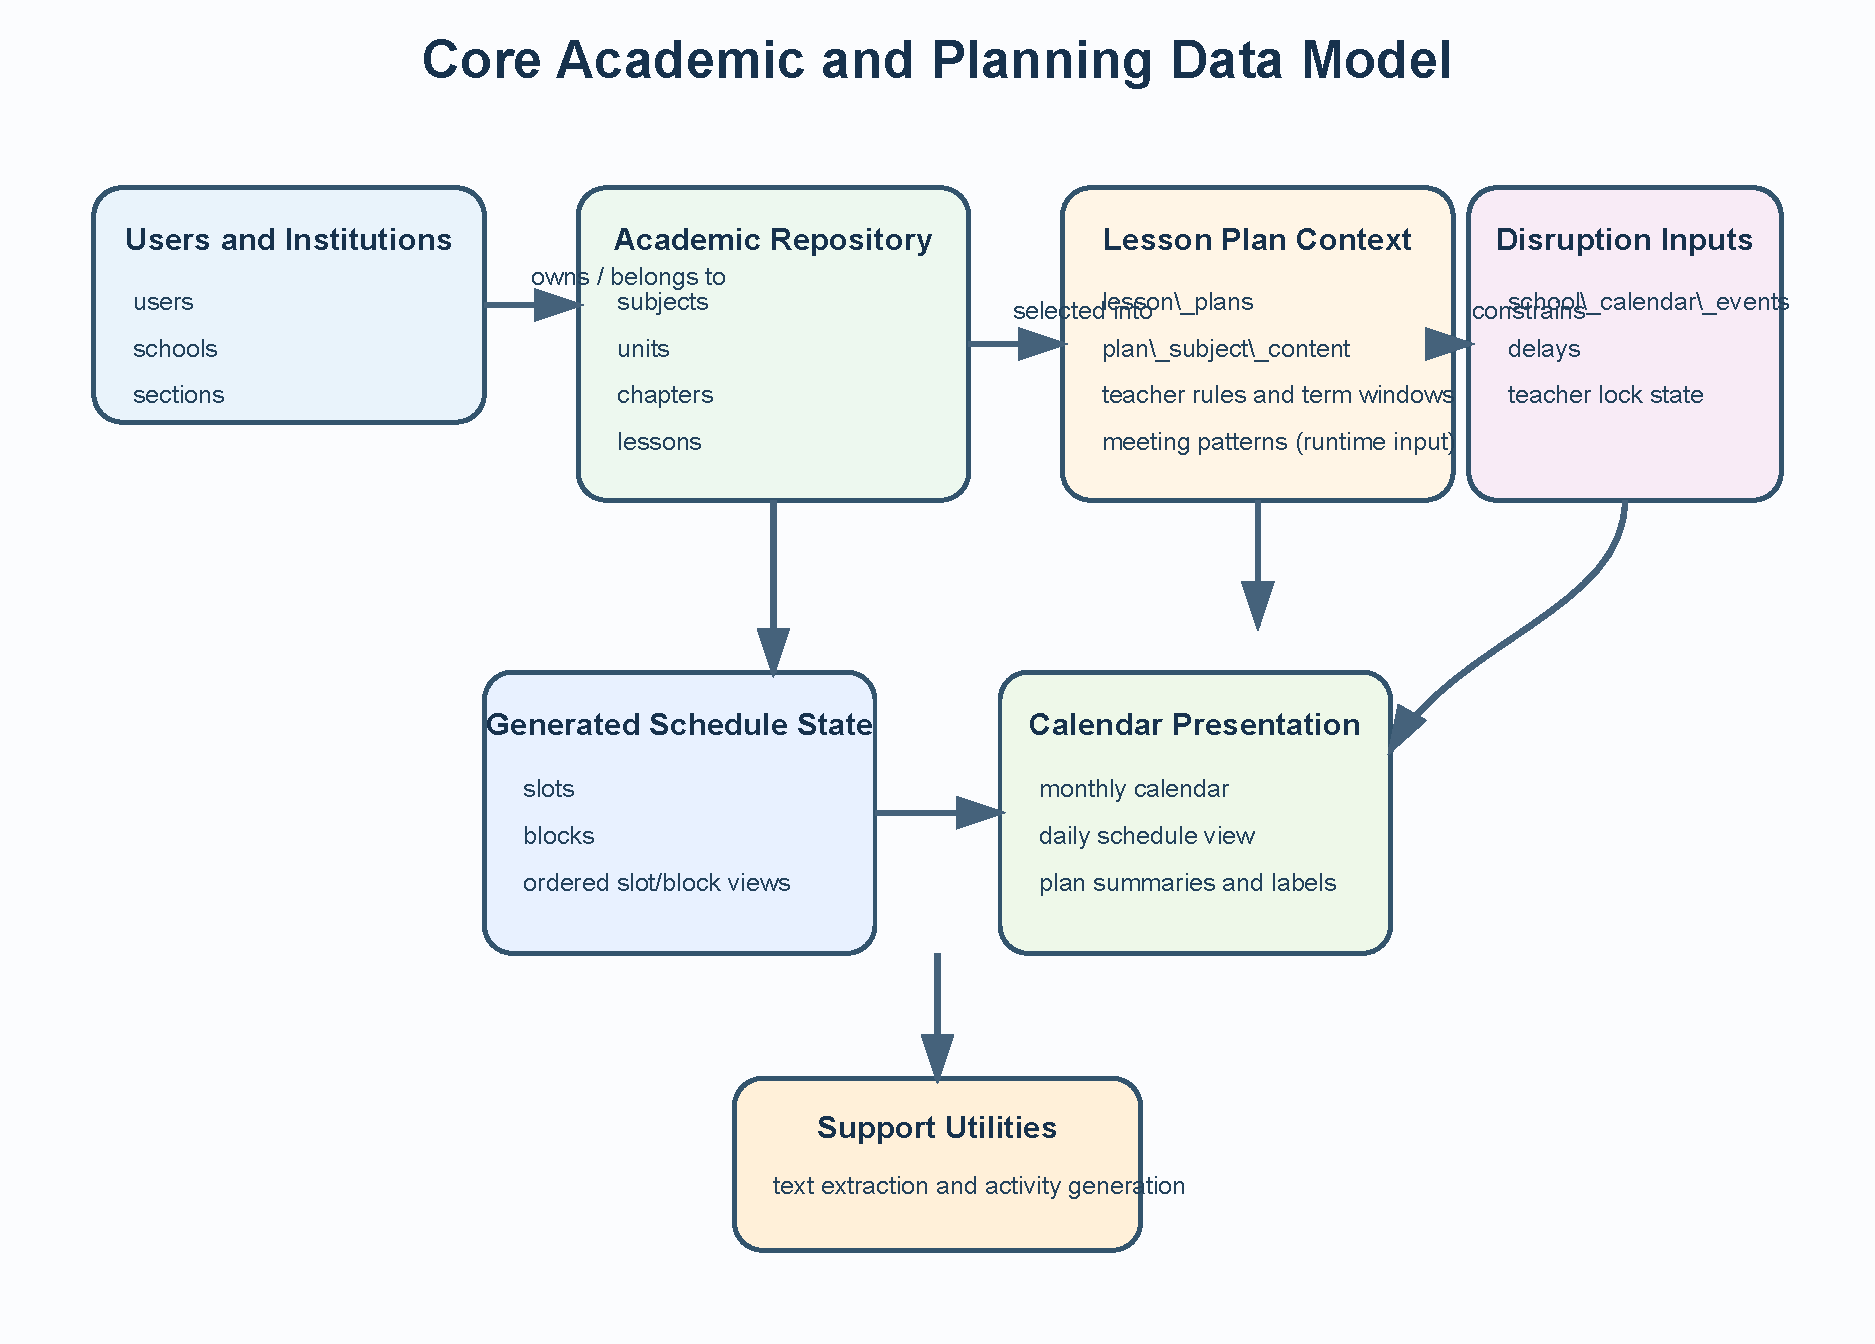
\includegraphics[width=0.48\textwidth]{figures/data-model.pdf}
\caption{Core academic and planning data model}
\label{fig:data-model}
\end{figure}

As shown in Figure~\ref{fig:data-model}, the model bridges two domains. The first
is the academic repository domain, which captures institutions, subjects, and
instructional content. The second is the planning-state domain, which captures how
that content is scheduled for a specific teacher and section over time. This bridge
is what enables the scheduler to operate on semantically meaningful content rather
than anonymous time blocks.

\subsection{Mobile Frontend Workflows}

The frontend exposes five major workflow areas. First, authentication and profile
screens manage sign-in, account settings, and institution membership. Second, the
library screens allow teachers to browse and maintain subjects and lesson content.
Third, the lesson-plan creation flow collects institutions, sections, term dates,
meeting patterns, and selected lesson scope. Fourth, the calendar screens visualize
the resulting schedule in monthly and daily forms. Fifth, creation utilities allow
teachers to upload curriculum materials and generate assessment documents.

This workflow design reflects the practical sequence in which teachers work: define
the context, encode the curriculum, generate the plan, inspect the calendar, and
adjust supporting materials as needed.

At the interface level, the workflow is distributed across authenticated route
groups and tab-based navigation. Profile and institution screens maintain user
context, the library screens maintain subject content, the create flow collects
planning constraints, and the calendar screens present schedule outputs. This
modular interface design mirrors the backend separation between identity, academic
repository data, and generated scheduling state.

\subsection{Live Demonstration Workflow}

The implemented system supports a defense demonstration that follows the same
sequence as normal teacher use. The presenter can sign in, open the profile and
institution context, create or load a subject with lessons, create a lesson plan
with meeting patterns and term settings, generate the schedule, and inspect the
result in plan and calendar views. The demonstration can then introduce a
class-day disruption, such as a suspension or delay, and show how SchEDU re-flows
non-locked blocks while preserving protected schedule state. A teacher-pinned
block that becomes infeasible is not silently moved; it remains visible as a
conflict requiring teacher re-pin action.

The same demo can also show the supporting document workflows. Curriculum files
can be uploaded for extraction into editable text, while written-work or
performance-task drafts can be generated through the activity workflow and
exported when the necessary backend services are configured. These services are
presented as teacher-assistance utilities, not as replacements for teacher
review or final instructional judgment.

\subsection{Rule-Based Scheduling Pipeline}

SchEDU uses a deterministic constraint-based greedy scheduler rather than a
search-based optimization engine. A single run consumes lesson-plan context,
recurring meeting patterns, selected lessons, stored activity requirements,
school calendar events, teacher-delay records, rule settings, and any existing
slot or block state that must be preserved. It returns four principal artifacts:
runtime slots, runtime blocks, a per-term schedule plan, and ordered
calendar-ready output, together with warnings and summary metrics. The
methodology is constructive: it first builds a feasible scheduling surface, then
derives term-aware block queues, then performs greedy placement, and finally
normalizes or rebalances the result. Because each stage is a pure function of
the current input state, repeated execution over unchanged inputs is
deterministic.

\begin{figure}[t]
\centering
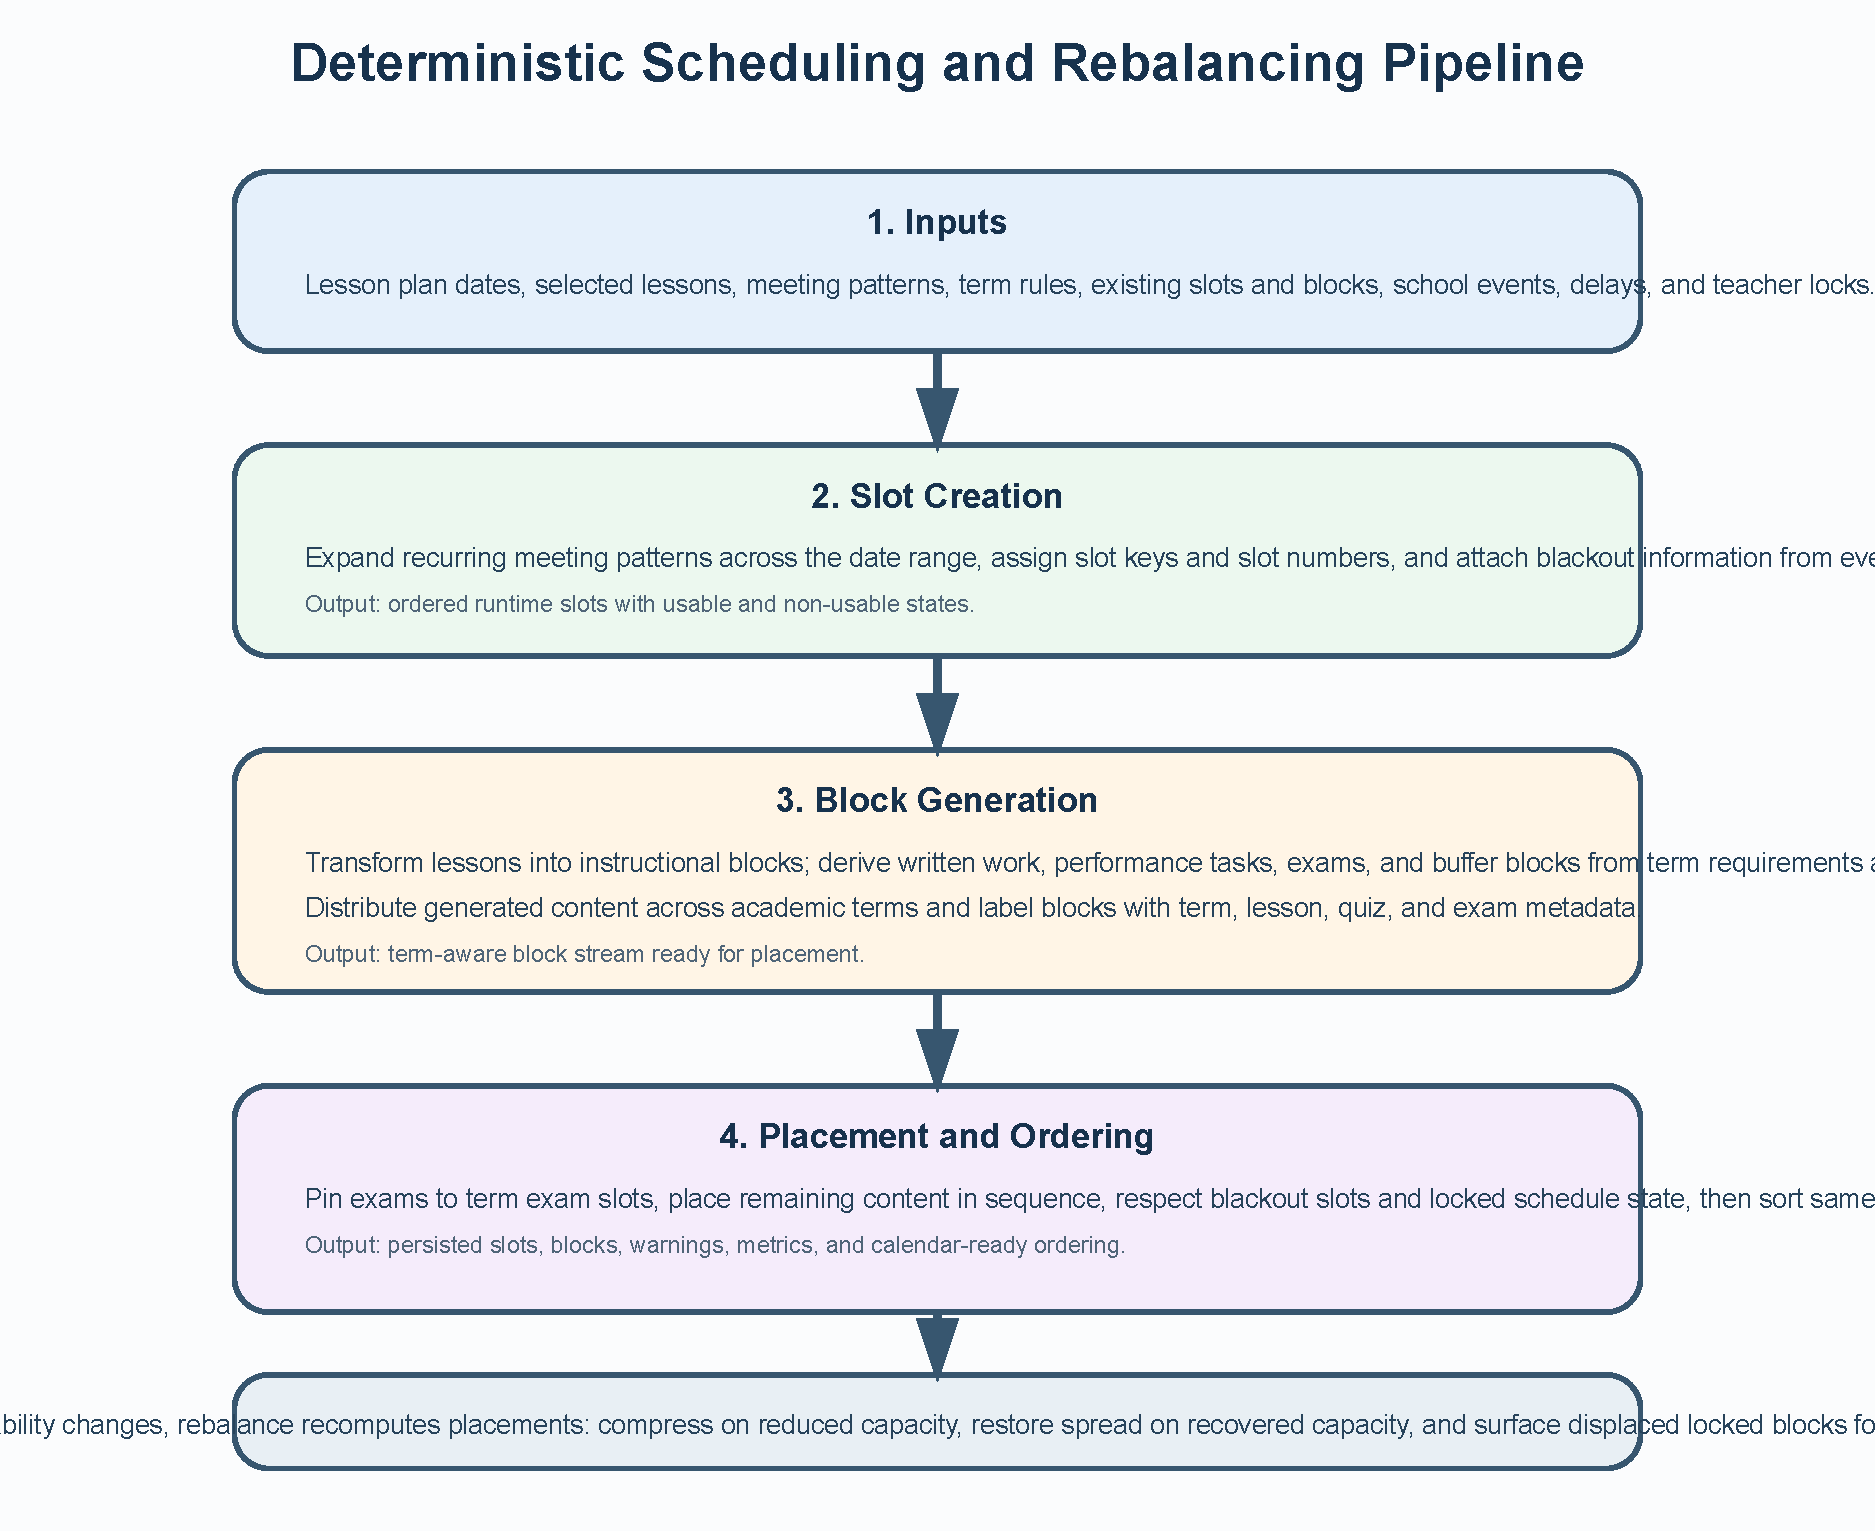
\includegraphics[width=0.48\textwidth]{figures/scheduler-pipeline.pdf}
\caption{Deterministic scheduling and rebalancing pipeline}
\label{fig:pipeline}
\end{figure}

Figure~\ref{fig:pipeline} summarizes the runtime flow from planning inputs to
calendar-ready outputs. The scheduler consumes structured records and rule
settings, derives slots and blocks in memory, partitions the schedule by term,
applies greedy placement logic, and finally exposes ordered outputs that can be
persisted and rendered by the calendar components.

\subsubsection{Theoretical Framing and Formal Model}

At the theory level, SchEDU can be described as a constrained activity-to-slot
assignment problem specialized for teacher pacing rather than institution-wide
timetabling \cite{schaerf1999}. Let the planning horizon be the set of dates
\(\mathcal{D}\) between the lesson-plan start date and end date, let
\(\mathcal{P}\) be the set of recurring meeting patterns, and let
\(\mathcal{B}\) be the set of schedulable blocks derived from lessons and
assessment rules. The scheduler constructs a feasible mapping
\(\phi : \mathcal{B} \rightarrow \mathcal{S} \cup \{\emptyset\}\), where
\(\mathcal{S}\) is the generated slot set and \(\emptyset\) denotes a block
that could not be placed under the current usable capacity.

The generated slot set is defined by date-pattern expansion:
\begin{equation}
\mathcal{S} =
\left\{
s_{d,j}
\;\middle|\;
d \in \mathcal{D},
\ \operatorname{weekday}(d)=p_j^{(w)},
\ p_j \in \mathcal{P}
\right\}.
\end{equation}
Each slot \(s_{d,j}\) stores a normalized start time, end time, meeting type,
slot number, series key, and date-specific slot key. A slot is usable only if it
is neither blacked out nor protected against scheduling:
\begin{equation}
u(s)=
\begin{cases}
1, & \neg blackout(s) \land \neg locked(s),\\
0, & \text{otherwise}.
\end{cases}
\end{equation}

The hard constraints enforced by the implementation are feasibility-oriented
rather than objective-oriented:
\begin{enumerate}
\item meeting-pattern end time must be later than start time;
\item meeting patterns on the same weekday must not overlap;
\item only usable slots may receive newly placed content blocks;
\item every term must have an exam anchor slot, whether existing or synthetic;
\item block-category and block-subcategory pairings must remain valid; and
\item compressed placement must respect slot capacity \(C=2\).
\end{enumerate}

Instead of optimizing a global cost function, the method uses deterministic
ordering and local feasibility rules. This is why the scheduler is better
described as constructive greedy scheduling under hard constraints than as
metaheuristic search.

\subsubsection{Slot Creation}

The system first creates candidate schedule slots from the lesson-plan date range
and recurring meeting patterns. Each meeting pattern specifies a weekday, a time
interval, an optional meeting type, and an inferred or explicit slot number.
Patterns are normalized by weekday and sorted by start time, then validated so
that overlapping class instances on the same day are rejected before planning
continues. The normalized patterns are expanded across every date in the lesson
plan, producing dated runtime slots with stable slot keys and series keys.

Calendar blackouts are then applied using school events and recorded delays such
as suspension, leave, or holiday entries. When an existing slot already exists in
storage, its persisted state can be merged back into the generated slot, allowing
manual lock state and prior identifiers to survive regeneration. If a locked slot
exists inside the plan window but is no longer regenerated from current meeting
patterns, it may still be preserved as part of the current scheduling surface.
The result is therefore more than a list of dates: it is a validated, constrained
calendar surface on which later scheduling decisions depend.

This stage gives the scheduler a deterministic temporal lattice. For any given
planning horizon and meeting-pattern set, slot generation is fixed before content
placement begins. That property is important because later stages reason over slot
keys, slot ordering, and blackout-adjusted usability rather than over free-form
calendar intervals.

\subsubsection{Block Generation}

The system next generates schedule blocks from lesson content and teacher rules.
The plan is first partitioned into academic terms ending on configured exam
dates. Usable slots are grouped term by term, and each term is assigned an exam
slot. If no regular class meeting exists on an exam date, the scheduler creates a
special synthetic exam slot so that the term still has a valid terminal anchor.
If \(e_k\) denotes the exam date for term \(k\), the usable content surface of
that term is bounded by
\begin{equation}
\mathcal{T}_k=
\left\{
s \in \mathcal{S}
\;\middle|\;
u(s)=1,\;
e_{k-1}<\operatorname{date}(s)\le e_k
\right\}.
\end{equation}
The exam anchor itself is selected by
\begin{equation}
s_k^{exam}=
\begin{cases}
\text{latest regular slot on } e_k, & \exists s:\operatorname{date}(s)=e_k,\\
\text{synthetic exam slot}, & \text{otherwise}.
\end{cases}
\end{equation}

Lessons become instructional blocks, while written work, performance tasks, exam
blocks, and buffer blocks are derived from term configuration and stored activity
requirements. Lesson blocks are distributed across terms by equal baseline
allocation, with any remainder assigned to earlier-priority terms first. The same
deterministic split rule is used for written-work and performance-task totals.
If \(L\) is the total lesson count and \(m\) is the number of terms, then the
per-term lesson count follows:
\begin{equation}
L_k=\left\lfloor \frac{L}{m} \right\rfloor + r_k,
\qquad
\sum_{k=1}^{m} r_k = L \bmod m,
\end{equation}
where the remainder indicators \(r_k\) are assigned to earlier-priority terms
first. The same pattern is used for written work and performance tasks.

Quiz blocks are then generated from scoped lesson groups and linked to their
prerequisite lesson blocks through dependency keys. In the current implementation,
the number of quizzes in term \(k\) is limited by both lesson coverage and the
written-work budget:
\begin{equation}
Q_k=\min \left(\left\lfloor \frac{L_k}{2} \right\rfloor, WW_k \right).
\end{equation}
The remaining non-quiz written work is therefore
\begin{equation}
\widetilde{WW}_k = WW_k - Q_k.
\end{equation}

To spread assessments across lesson progression, the scheduler computes interval
values from the lesson and assessment counts:
\begin{equation}
\Delta^{ww}_k=
\begin{cases}
\max\left(1,\left\lfloor \frac{L_k}{\widetilde{WW}_k}\right\rfloor\right), & \widetilde{WW}_k > 0,\\
0, & \text{otherwise},
\end{cases}
\end{equation}
\begin{equation}
\Delta^{pt}_k=
\begin{cases}
\max\left(1,\left\lfloor \frac{L_k}{PT_k}\right\rfloor\right), & PT_k > 0,\\
0, & \text{otherwise}.
\end{cases}
\end{equation}
These intervals are stored as term metadata and later consumed by the placement
state machine. Each generated block also carries term-aware metadata including
term key, term number, exam date, exam slot key, lesson number, and quiz scope
summary. The first term may prepend an orientation buffer block before regular
instruction begins.

This stage is what translates pedagogical content into schedulable units. Lessons
retain content identity through metadata, while assessments are derived according
to pacing rules rather than inserted as arbitrary placeholders. The system
therefore preserves the relationship between curriculum coverage and later
calendar placement.

\subsubsection{Placement and Ordering}

Generated blocks are then placed onto slots according to term structure and
category-specific rules. For each term, the scheduler builds explicit queues for
lessons, quizzes, other written work, performance tasks, exams, and buffer
blocks. It reserves the exam slot first, then places the orientation buffer if
the opening term has surplus capacity, and then walks the content-slot sequence
chronologically.

Each lesson consumes the next usable untaken content slot. After each lesson
placement, the scheduler checks whether any quiz dependencies have been satisfied;
if so, the due quiz blocks are released immediately after the covered lesson
sequence. The scheduler also checks interval counters for written work and
performance tasks, allowing those categories to enter the calendar at regular
curriculum-driven points rather than at arbitrary dates. This is the greedy core
of the method: at each step, the next feasible slot and the next due block are
chosen deterministically, without backtracking.

The greedy selection rule can be written as
\begin{equation}
\phi(b_i)=
\arg\min_{s \in A(b_i)}
\bigl(\operatorname{date}(s),\operatorname{start}(s),\operatorname{slotNo}(s)\bigr),
\end{equation}
where \(A(b_i)\) is the feasible candidate set for block \(b_i\) at the current
step. For lessons, this feasible set is the next chronological usable content
slot that is not already occupied by preserved state. For quizzes, feasibility is
also conditioned on prerequisite satisfaction:
\begin{equation}
ready(q)=1
\iff
Dep(q)\subseteq P_L,
\end{equation}
where \(Dep(q)\) is the set of lesson-block dependencies attached to quiz \(q\)
and \(P_L\) is the set of already placed lesson blocks in the current term.

If a term is overcommitted, the placement logic applies bounded compression
heuristics rather than abandoning the plan. Non-quiz written work prefers to ride
along the current or latest lesson slot with available capacity. Performance tasks
first prefer a lesson slot that does not already contain written work, then fall
back to any compatible lesson slot with room. If no feasible slot remains, the
block is left unplaced and the scheduler emits warnings rather than silently
dropping it.

The implementation measures overcommitment through slot pressure:
\begin{equation}
\rho_k = |\mathcal{B}^{content}_k| - |\mathcal{U}^{content}_k|,
\end{equation}
where \(\mathcal{B}^{content}_k\) is the set of lesson, written-work, and
performance-task blocks in term \(k\), and \(\mathcal{U}^{content}_k\) is the set
of usable non-exam slots in that term. A positive \(\rho_k\) indicates that
compression is required. The dual quantity,
\begin{equation}
\epsilon_k = |\mathcal{U}^{content}_k| - |\mathcal{B}^{content}_k| = -\rho_k,
\end{equation}
represents excess slot capacity. During compression, the feasibility condition for
any candidate host slot \(s\) must satisfy
\begin{equation}
occ(s) < C, \qquad C = 2,
\end{equation}
where \(occ(s)\) is the current number of blocks assigned to the slot.

After placement, blocks sharing a slot are ordered and re-numbered so that the
calendar display remains stable and interpretable. Within-slot ordering follows a
fixed reading priority: orientation first, then lesson, written work,
performance task, buffer, and exam. The placement stage also computes warnings
and plan-level metrics, which are useful for surfacing incomplete or
overcommitted configurations.

\subsubsection{Rebalancing Under Disruption}

When a class day becomes unavailable or available again, the scheduler performs a
rebalancing pass. Rebalancing treats schedule maintenance as deterministic
re-flow. Teacher-locked blocks, exam blocks, and buffer blocks are treated as
pinned state. Non-pinned blocks are first released from their previous
assignments, the term schedule plan is recomputed from the currently usable
slots, live term balance is recalculated, and the placement pass is executed
again while respecting any surviving pinned placements.

If \(P\) denotes the pinned block set, then the pinned-state rule is
\begin{equation}
P=\left\{b \in \mathcal{B}\ \middle|\ locked(b)\ \lor\ cat(b)\in\{\text{exam},\text{buffer}\}\right\}.
\end{equation}
Rebalancing can then be viewed as
\begin{equation}
R(X)=Place\bigl(Release(X \setminus P),\;P\bigr),
\end{equation}
where \(X\) is the current schedule state. In other words, the scheduler releases
all non-pinned content, recomputes term balance from the currently usable slot
surface, and greedily places the released blocks again around the surviving
pinned assignments.

This enables both directions of maintenance. If usable capacity shrinks, the
placement heuristics compress assessments onto compatible lesson slots. If
capacity is restored, the same deterministic pass can spread blocks back out
without requiring a separate undo log. A teacher-locked block whose day became
unusable is not auto-moved. Instead, it is kept locked but unplaced, reported as
a conflict, and paired with suggested re-pin candidates so that teacher intent is
preserved and the unresolved decision remains visible.

This rebalance behavior is one of the system's most practical features. It treats
schedule change as a state-maintenance problem: preserve teacher intent where
possible, recompute what is flexible, and expose any unresolved conflict rather
than silently discarding data. Because rebalance is a pure function of the
current state, applying it twice to an unchanged schedule is idempotent:
\begin{equation}
R(R(X)) = R(X).
\end{equation}
For teacher use, this is more valuable than a one-time initial schedule because
academic plans often change after they have already been prepared.

\subsection{Auxiliary Services}

Two support services extend the planning workflow. The first is curriculum text
extraction: PDF or image files can be uploaded, stored, and processed into editable
text for curriculum encoding. The second is AI-assisted activity generation:
teachers can define category, scope, components, and template guidance, and the
system returns classroom-ready written-work or performance-task drafts. These
services are not the core scheduling engine, but they reduce manual preparation
work around it.

Together, these services expand SchEDU from a scheduler into a broader planning
workspace. Curriculum extraction reduces the cost of encoding source materials into
structured lessons, while activity generation shortens the path from scheduled
content to assessable classroom outputs. This is consistent with the paper's system
focus: the scheduler is central, but it is embedded in a wider teaching workflow.

\section{Scheduler Behavior and Validation}

The scheduler is validated through executable invariants and repository-backed
usage flows rather than benchmarked against mathematical objective scores. This
validation strategy is appropriate because the implemented scheduler is
deterministic and rule-based. The primary question is not whether a global optimum
is achieved, but whether the generated and maintained plan remains consistent,
recoverable, and usable under realistic teacher actions.

The invariant checks cover initial plan generation, blackout handling, schedule
compression during suspension, restoration after unsuspension, idempotent rebalance
behavior, and the displacement flow for teacher-locked blocks that become
conflicted. In the current repository state, the command \texttt{npm run
test:scheduler} completes with all invariant checks passing. Static validation
through \texttt{npm run lint} completes with no errors and seven warnings. The
warnings are treated as quality debt rather than blocking defects because they are
unused variables, array-style guidance, and a byte-order-mark warning.

Validation of the broader application combines source-backed workflow tracing and
live demonstration. Authentication and protected route behavior are backed by
Supabase Auth usage in the app. Persistence claims are backed by schema definitions
for users, schools, sections, subjects, lessons, lesson plans, selected content,
slots, blocks, calendar events, delays, and activities. The document utilities are
guarded by authenticated Edge Functions: extraction requires a bearer token and
user-owned storage path, while activity generation validates the request before
returning generated text.

\begin{table*}[t]
\centering
\caption{Implementation Evidence Used for Defense Readiness}
\label{tab:evidence}
\begin{tabular}{>{\raggedright\arraybackslash}p{0.20\textwidth}>{\raggedright\arraybackslash}p{0.37\textwidth}>{\raggedright\arraybackslash}p{0.34\textwidth}}
\toprule
Evidence area & Repository-backed evidence & Defense relevance \\
\midrule
Scheduler invariants & \texttt{npm run test:scheduler} passes initial generation, suspension, restoration, idempotency, locked-block conflict, and re-pin checks. & Demonstrates that the core scheduling claim is executable and not only descriptive. \\
\addlinespace
Static validation & \texttt{npm run lint} completes with zero errors and seven non-blocking warnings. & Shows that the current codebase is lintable while documenting remaining quality debt honestly. \\
\addlinespace
Persistence model & Supabase schema covers academic repository data, planning state, slots, blocks, calendar events, delays, and generated activities. & Supports the claim that demo data survives across workflows instead of existing only in UI state. \\
\addlinespace
Security guards & Authenticated routes, RLS-oriented schema setup, storage ownership paths, and bearer-token Edge Functions protect sensitive flows. & Supports a defensible security baseline for account and document workflows. \\
\addlinespace
Live workflow coverage & App routes cover authentication, profile, institution, library, lesson-plan creation, plans, calendar, daily agenda, admin, extraction, and activity generation. & Lets panel members observe the system as a full workflow during the live demo. \\
\bottomrule
\end{tabular}
\end{table*}

\section{Results and Discussion}

\subsection{Implementation Validation Scenarios}

Table~\ref{tab:validation} summarizes validation scenarios supported by the current
repository implementation. These scenarios were selected because they correspond
to the most failure-prone parts of a live defense demonstration: generation,
disruption, restoration, and preservation of teacher intent.

\begin{table*}[t]
\centering
\caption{Repository-Supported Validation Scenarios}
\label{tab:validation}
\begin{tabular}{>{\raggedright\arraybackslash}p{0.20\textwidth}>{\raggedright\arraybackslash}p{0.35\textwidth}>{\raggedright\arraybackslash}p{0.35\textwidth}}
\toprule
Scenario & Expected behavior & Observed system response \\
\midrule
Initial plan generation & Lessons and required assessments are placed across generated meeting slots without losing blocks. & The scheduler produces a complete initial plan with ordered slots and placed blocks, while exposing plan metrics and warnings when needed. \\
\addlinespace
Blackout or delay handling & Slots affected by school events or teacher delays become unavailable to normal placement. & Blackout information is attached to slots and considered during generation and rebalance passes. \\
\addlinespace
Suspension of a teaching day & When one usable day is suspended, remaining blocks are re-flowed without data loss. & Rebalancing compresses the plan into remaining usable slots and preserves total block count. \\
\addlinespace
Unsuspension and restoration & When a suspended day becomes available again, the plan should recover to a stable layout. & Rebalancing after unsuspension removes temporary compression and can restore the original block layout. \\
\addlinespace
Idempotent maintenance & Re-running rebalance on an already stable plan should not introduce drift. & A repeated rebalance acts as a no-op for an already balanced schedule state. \\
\addlinespace
Teacher-locked block conflict & A teacher-pinned block on a newly suspended day should not silently disappear. & The locked block is displaced, surfaced for re-pinning, and accompanied by suggested placement options rather than being discarded. \\
\bottomrule
\end{tabular}
\end{table*}

\subsection{Live Demonstration Readiness}

The implemented application supports a coherent defense walkthrough. The strongest
path is to begin with a prepared authenticated teacher account, open existing
institution and subject records, create or load a lesson plan, generate schedule
state, and then inspect the result in the calendar. This avoids spending the
limited presentation time on repeated data entry while still demonstrating that
the data model, UI, and scheduler are connected.

A recommended demonstration sequence is as follows. First, show account access and
profile or institution context. Second, open the subject library and show lessons
that can become schedule input. Third, generate or load a lesson plan with meeting
patterns and term settings. Fourth, inspect the monthly and daily calendar views.
Fifth, suspend or restore a class day to show rebalance behavior. Sixth, open an
activity or extraction workflow to show document support. Seventh, open the
administrative dashboard if an authorized demo account is available.

Several dependencies must be controlled for the live presentation. Supabase
credentials must point to a provisioned project, the schema and policies must be
applied, and demo records should be prepared beforehand. Image OCR requires a
native-capable development build rather than Expo Go. AI-assisted activity
generation depends on backend service configuration, so prepared records or
screenshots should be available if external service availability interrupts that
portion of the demonstration.

\subsection{Discussion}

The implemented behavior shows that SchEDU is most appropriately understood as a
teacher planning system with built-in schedule maintenance logic. Its value lies in
keeping academic content, schedule state, and supporting documents within a shared
data model. This reduces the gap between planning and execution: changes in
institutional context, such as suspended classes or delayed meetings, can be
processed within the same system that stores the lessons and assessments affected by
those changes.

The rule-based approach also offers practical advantages for a teacher-facing tool.
Because the scheduler is deterministic, repeated runs under the same inputs produce
consistent outcomes, making the system easier to inspect and debug. This is
important in planning contexts where teachers may need to understand why a block was
placed, moved, compressed, or displaced.

At the same time, the current validation remains implementation-centered. The
repository demonstrates functional scheduling behavior and maintenance guarantees,
but it does not yet provide large-scale empirical studies, user acceptance results,
or comparative evaluations against other planning systems. The appropriate defense
claim is therefore that SchEDU is a working, demo-ready academic planning system
with validated scheduler behavior, not that it is a fully production-certified
learning management platform.

\section{Conclusion}

This paper presented SchEDU as an implemented mobile academic planning and
rule-based scheduling system for teachers. The system integrates structured
curriculum storage, lesson-plan creation, schedule generation from recurring
meeting patterns, calendar rebalancing under disruptions, curriculum text
extraction, and AI-assisted activity document support within a unified mobile
workflow.

The implementation demonstrates that teacher planning can be treated as a connected
data-and-scheduling problem rather than a collection of isolated documents and
calendar entries. By linking academic content, term rules, class meetings, and
disruption handling inside one system, SchEDU reduces the effort required to create
and maintain instructional plans.

From a systems perspective, SchEDU's main contribution is not a claim of formal
optimality but the integration of several planning responsibilities that are usually
fragmented across separate tools. The mobile interface gives teachers direct access
to planning workflows, the backend preserves institutional and curricular state, and
the scheduling pipeline converts that state into a maintainable calendar. This
combination is what makes the system practically useful: schedule generation is
grounded in real lesson content, and schedule maintenance remains connected to the
same records that teachers edit during normal academic work.

The detailed methodology also shows that instructional scheduling at the teacher
level benefits from deterministic, inspectable behavior. In SchEDU, meeting
patterns, lesson scope, blackout information, and term rules are transformed into
slots and blocks through explicit stages. As a result, the system can explain its
state transitions more clearly than a purely opaque scheduling engine. This matters
for adoption, because teachers need to trust that changes such as suspensions,
teacher absences, or manual schedule locks will be handled consistently.

The current implementation nevertheless has clear boundaries. The reported results
are implementation validations rather than large-scale field evaluations. The
repository demonstrates that the scheduler can generate plans, preserve blocks
under compression and restoration, and surface displaced locked items for manual
repair, but it does not yet establish broader pedagogical impact, long-term
usability, or institution-wide deployment outcomes. SchEDU should therefore be
presented as a defense-ready implemented prototype with a clear path toward
production hardening, not as a finished campus-wide scheduling or learning
management system. These limitations should be treated as part of the current
maturity of the system rather than as defects in the architectural approach.

Future work includes broader empirical evaluation, usability studies with teachers,
refinement of scheduler heuristics, stronger analytics for plan quality and progress
tracking, and tighter integration of administrative and cross-role planning
features. Additional work may also explore richer calendar editing operations,
improved curriculum-ingestion pipelines, and more structured evaluation of
AI-assisted document generation in actual classroom preparation contexts.

\begin{thebibliography}{10}

\bibitem{pak2020}
K. Pak, M. S. Polikoff, L. M. Desimone, and E. Sald{\'\i}var Garc{\'\i}a,
``The adaptive challenges of curriculum implementation,''
\emph{AERA Open}, vol. 6, no. 2, pp. 1--15, 2020.

\bibitem{schaerf1999}
A. Schaerf,
``A survey of automated timetabling,''
\emph{Artificial Intelligence Review},
vol. 13, no. 2, pp. 87--127, 1999.

\end{thebibliography}

\end{document}
